\begin{figure}[tb]
                       	\begin{center}
                       		\begin{tabular}{  c | c | c   }
                       			%\hline
                       			&\large{\textsf{$\bLambda$}}   &\large{\textsf{SAMPLES }} \hspace{.55in}   \\ \hline
                     
&\vspace{-.1in}& \\
                       			\multirow{1}{*}[.6in]{ \rotatebox[origin=t]{90}{\large{\textsf{a = 2}} }}
                                &
{{ 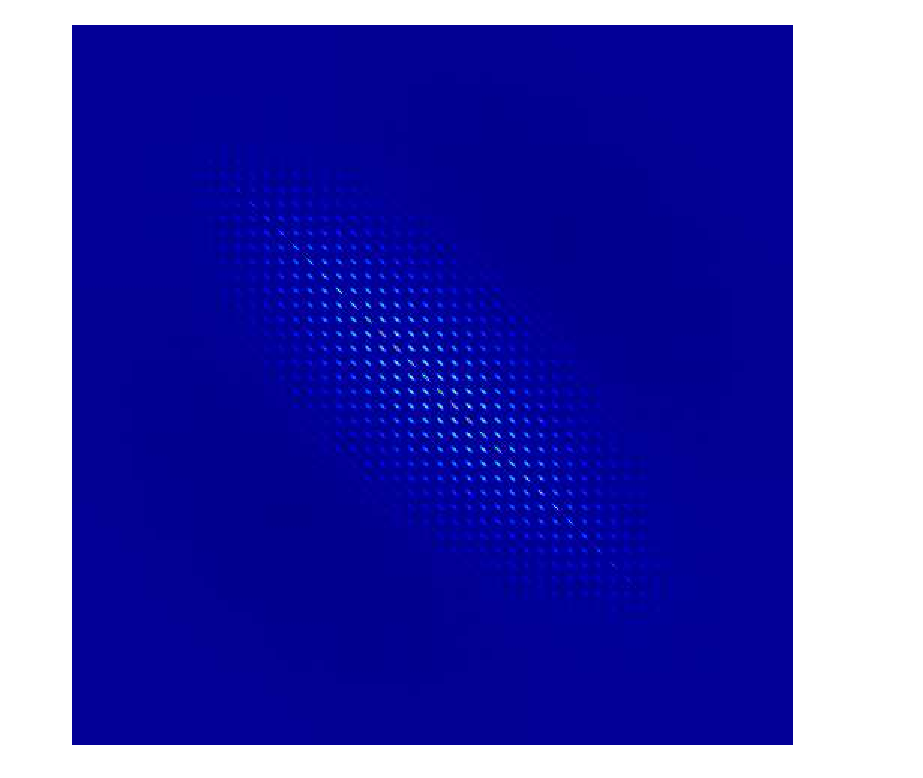
\includegraphics[width=0.2\linewidth]{figures/prior/outfile_drop2_cropped.pdf}} } &
                       			{ 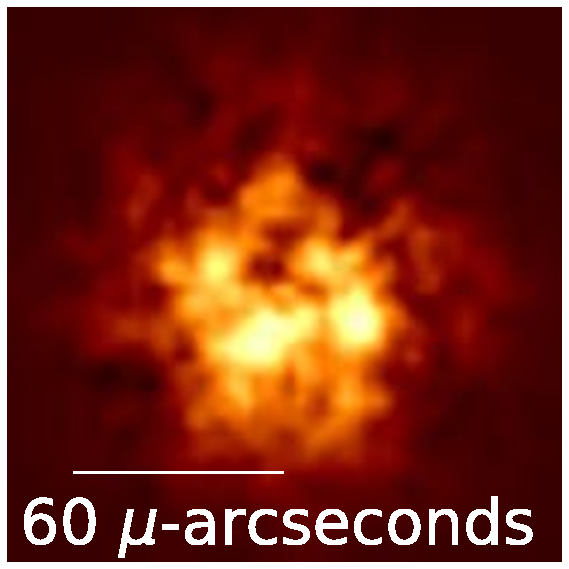
\includegraphics[width=0.2\linewidth]{figures/prior/newfiles/sampfig_drop2_1_scale2.pdf}} 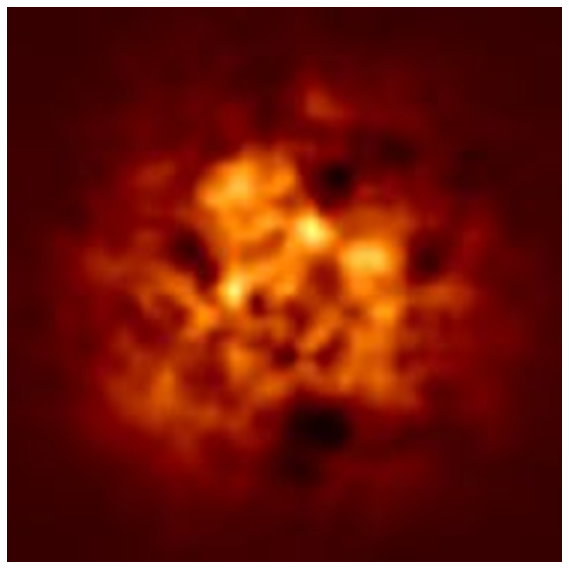
\includegraphics[width=0.2\linewidth]{figures/prior/newfiles/sampfig_drop2_4.pdf} 
                       			\multirow{3}{*}[.6in]{ 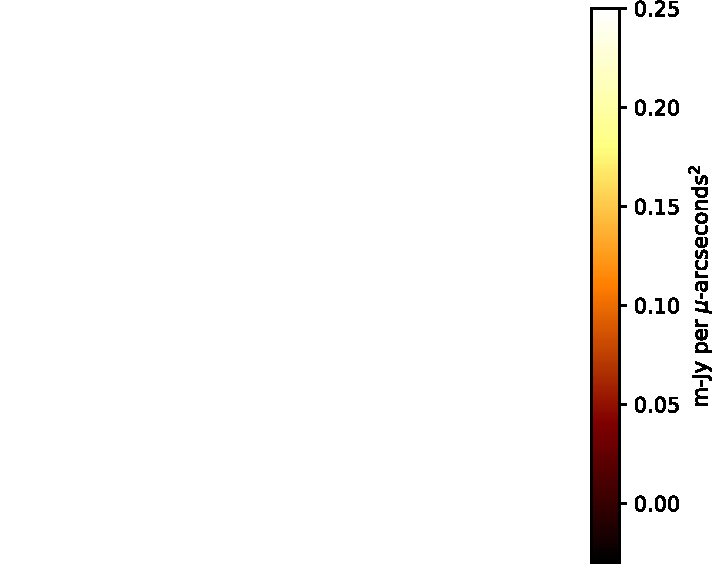
\includegraphics[width=0.155\linewidth]{figures/prior/newfiles/sampfig_drop2_1_cbar.pdf} }
                                \\
                       			&\vspace{-.1in}&\\
                       			\multirow{1}{*}[.6in]{ \rotatebox[origin=t]{90}{\large{\textsf{a = 3}} }} & 
                       			{{ 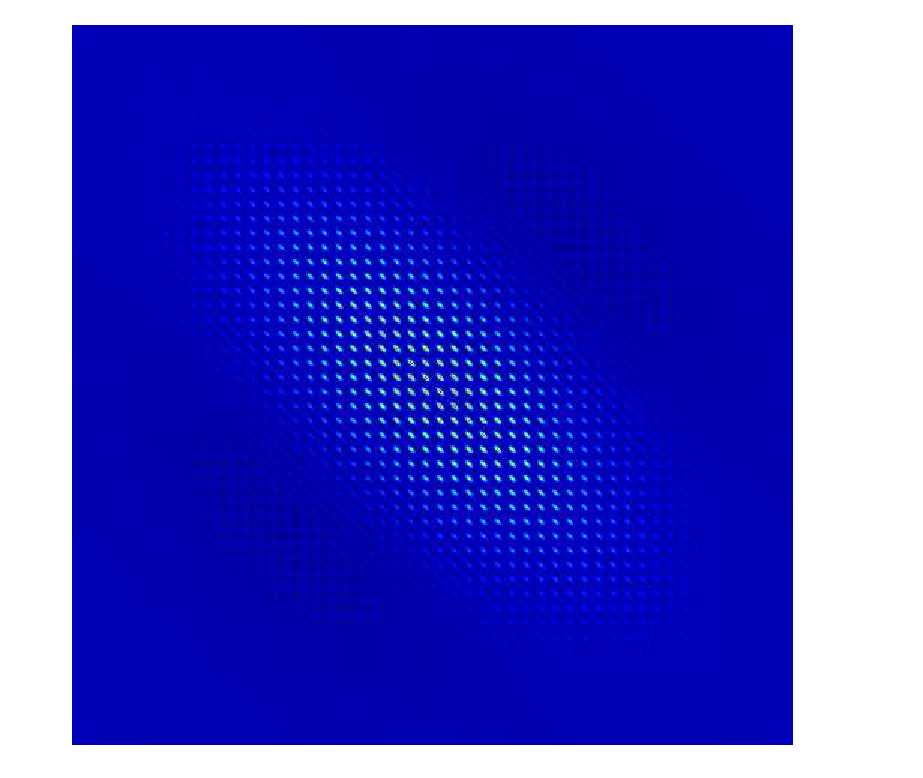
\includegraphics[height=0.2\linewidth]{figures/prior/outfile_drop3_cropped.pdf}} } &
                       			{ 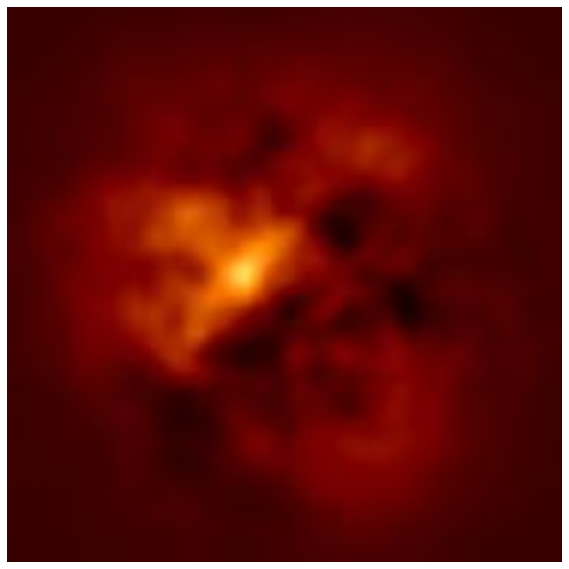
\includegraphics[height=0.2\linewidth]{figures/prior/newfiles/sampfig_drop3_2.pdf}} 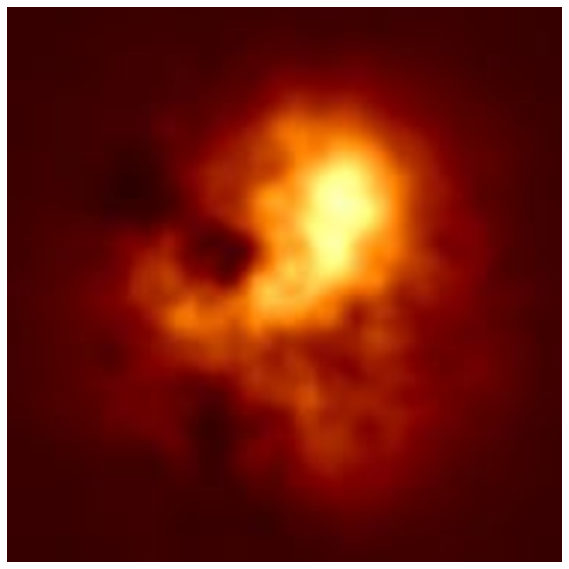
\includegraphics[height=0.2\linewidth]{figures/prior/newfiles/sampfig_drop3_3.pdf}  
                       			\hspace{.65in}
                       			%\multirow{3}{*}[.6in]{ 
\includegraphics[width=0.18\linewidth]{figures/prior/newfiles/placeholder.pdf} }
                       			\\
                       			&\vspace{-.1in}& \\
                       			\multirow{1}{*}[.6in]{ \rotatebox[origin=t]{90}{\large{\textsf{a = 4}} }} & 
                       			{{ 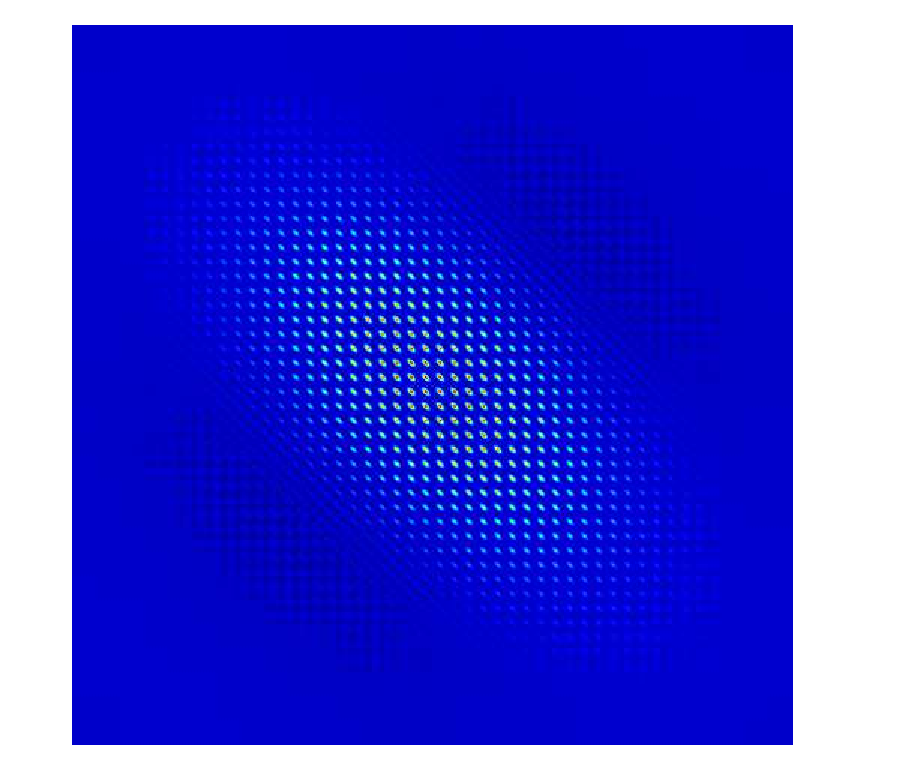
\includegraphics[height=0.2\linewidth]{figures/prior/outfile_drop4_cropped.pdf}} } &
                       			{ 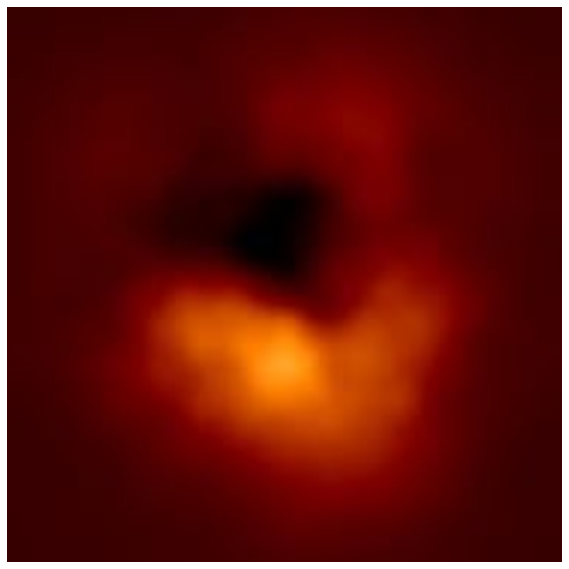
\includegraphics[height=0.2\linewidth]{figures/prior/newfiles/sampfig_drop4_1.pdf}} 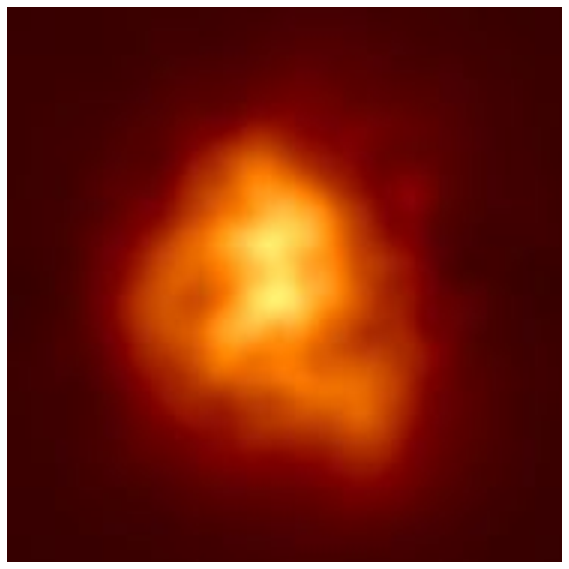
\includegraphics[height=0.2\linewidth]{figures/prior/newfiles/sampfig_drop4_2.pdf}                        			
                       			\hspace{.65in}
                       			%\multirow{3}{*}[.6in]{ 
\includegraphics[width=0.18\linewidth]{figures/prior/newfiles/placeholder.pdf} } 
                       			\\            	
                       		\end{tabular}
                       		\caption{\footnotesize{{\bf Gaussian Image Prior:} The covariance matrix constructed for $a=2,3,4$ along with image samples from the prior  $\mathcal{N}_x(\mu, \Lambda)$. The image samples have a field of view of 160 $\mu$-arcseconds. Notice that as $a$ increases, the sampled images appear smoother (i.e., the prior encourages smoother structure). In these examples $\mu$ is a 2D Gaussian image with standard deviation of 75 $\mu$-arcseconds. and $c=0.5$. 
                       			}}
                       			\label{fig:priorsamples}
\end{center}
\vspace{-.2in}
\end{figure}